\section{RAOES Implementation Method}
\label{sec:implementation}
%A prototype is implemented to realize our approach. 
This section presents the architecture and implementation detail of a RAOES prototype based on the Eclipse Modeling Framework (EMF).
The latter provides many facilities such to ease the development.
Fig. \ref{fig:architecture} shows the RAOES's architecture.
The latter consists of the C++ front-end extending C++, a synchronizer between the model and the front-end, and a source-to-source transformation.
The implementation of these modules is presented in the followings. 
Although some Eclipse facilities are used, the implementation method is generic and can be applied to other development environments.

\begin{figure}
	\centering
	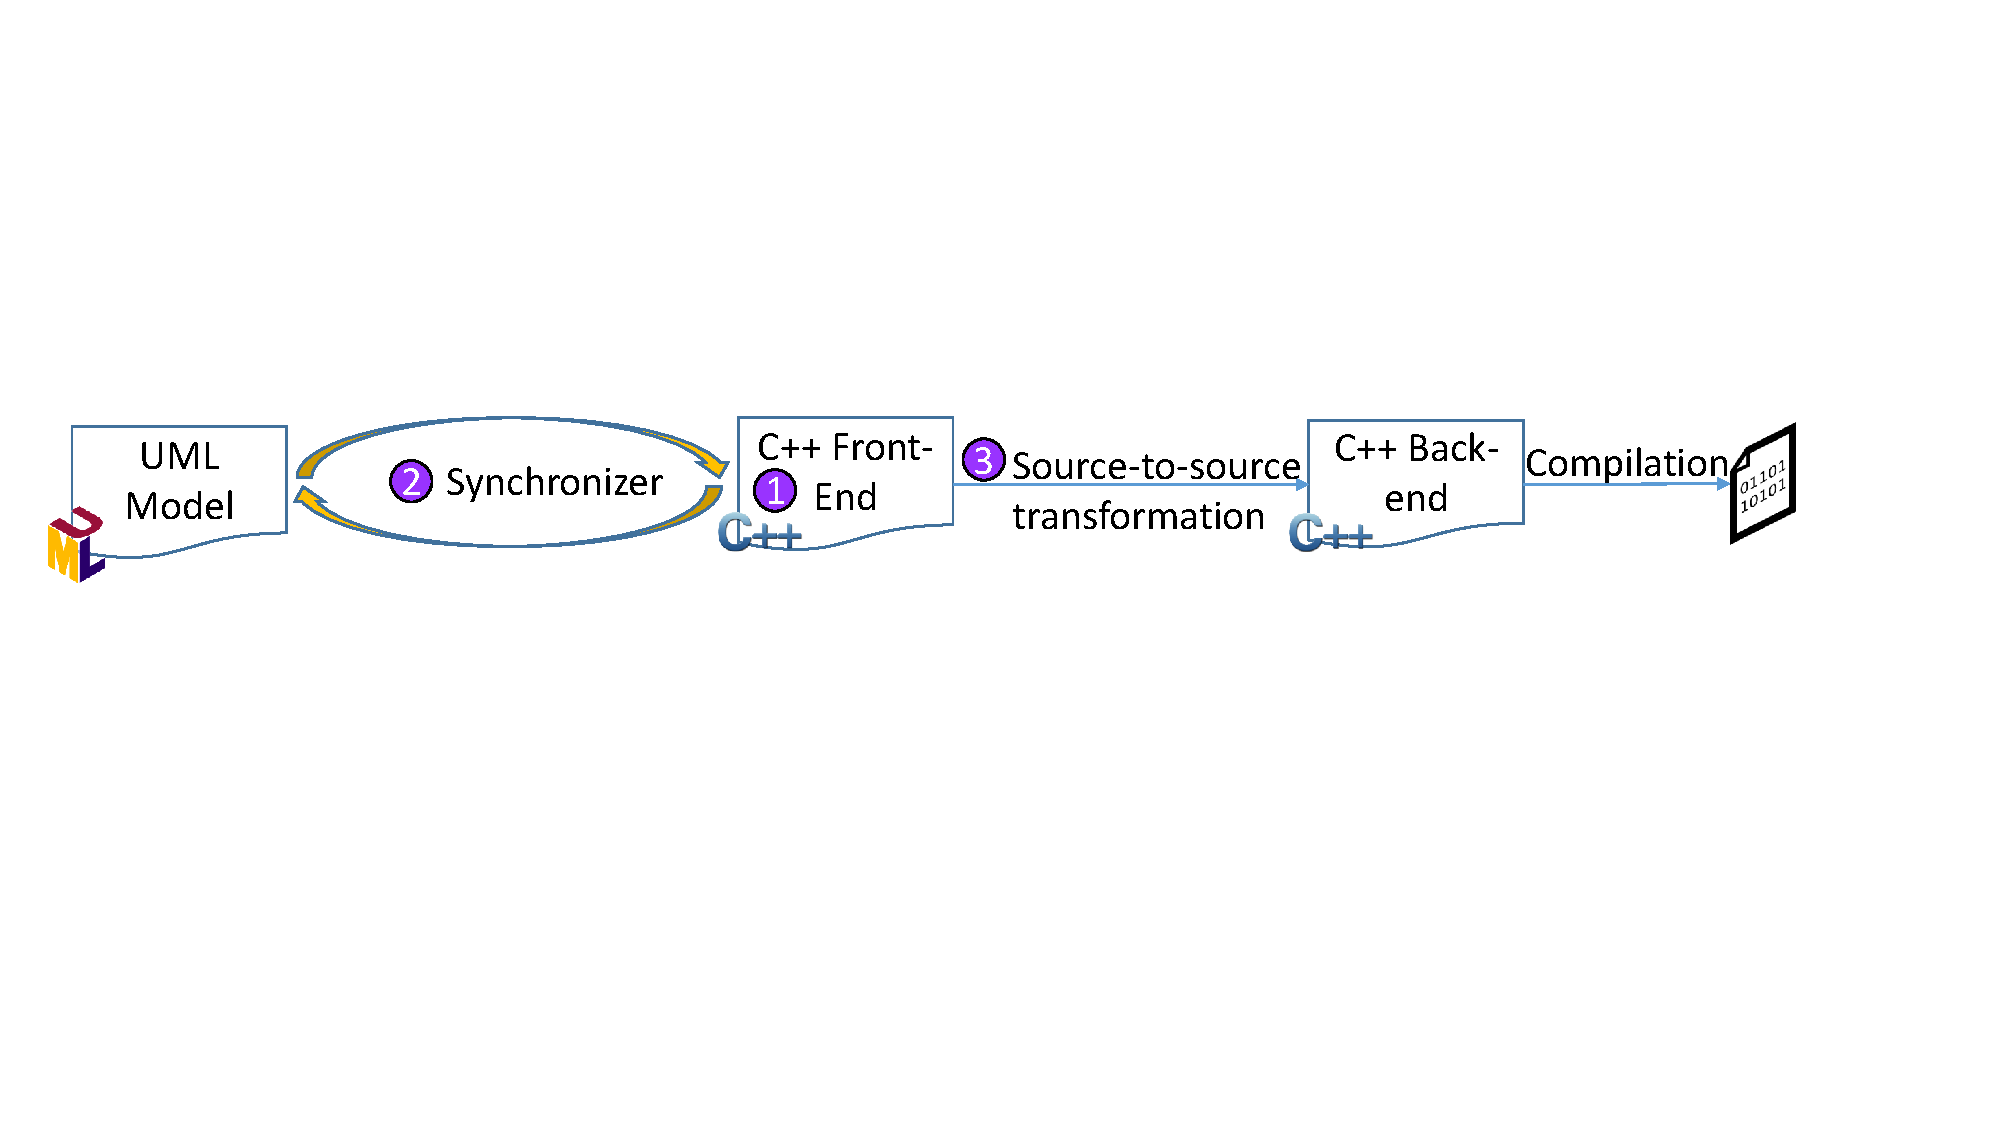
\includegraphics[clip, trim=0.8cm 9.5cm 3.2cm 6.8cm, width=1.0\columnwidth]{figures/architecture.pdf}
	\caption{RAOES's architecture} 
	\label{fig:architecture}
\end{figure}

\subsection{C++ front-end implementation}
The purpose of introducing the front-end is to ease and reduce the programmers' effort in modifying the topology of USMs, including all features.
%This front-end is then used by a source-to-source (C++-to-C++) transformation to generate a C++ back-end code.
Therefore, the front-end should be easily parsed by inspecting the \ttt{Abstract Syntax Tree (AST)} of C++.
The front-end is presented in a hierarchical way.
Hence, we use the class hierarchy in C++ to represent the underlying.
This is of course not the only one way to define the front-end.
%The underlying of some concepts in our implementation is shown in Listing \ref{lst:underlying}.
To easily recognize the state machine element types in RAOES, we use specialized names embedded in the macro definitions of RAOES. 

In this implementation, hierarchical elements such as \ttt{State Machine}, \ttt{State}, \ttt{Region} in concurrent states, and events are implemented as classes.
Pseudo states, which are contained by either a region or state (e.g. connection points), are implemented as class attributes.
Each transition is associated with a statement in a method representing the transition table.
By using this implementation, the front-end is compilable with C++ compilers such as GCC.

\begin{comment}
\begin{lstlisting}[float=*,language=C++, caption=The underlying representation of the C++ front-end, label=lst:underlying]
#define STATE(name,ent,ex)	class STATE___ ## name ## ___ ## ent ## ___ ## ex ## ___
#define INITIAL_STATE(name,ent,ex,effect) class INITIAL_STATE___ ## name ## ___ ## ent ## ___ \
											## ex ## ___ ## EFFECT ## ___ ## effect
#define REGION(name)	class REGION___ ## name ## ___
#define STATE_MACHINE(name)	class STATE_MACHINE___ ## name ## ___
#define CALL_EVENT(name,operation) class CALL_EVENT___ ## name ## ___OPERATION___ ## operation {};
#define TIME_EVENT(name,duration) class TIME_EVENT___ ## name ## ___DURATION___ ## duration {};
#define SIGNAL_EVENT(name,signal) class SIGNAL_EVENT___ ## name ## ___SIGNAL___ ## signal {};
#define SIMPLE_EVENT(name) class SIGNAL_EVENT___ ## name ## ___SIGNAL___NULL{}; 
#define CHANGE_EVENT(name,expression) class CHANGE_EVENT___ ## name ## ___EXPRESSION___ \
					{const char* func() {return #expression;}};
#define TRANSITION_TABLE void TRANSITION_TABLE___operation(int transition_len)
#define TRANSITION(source, target, guard, event, effect) transition_len = strlen("transition") + \
		strlen(#source) + strlen(#target) + strlen(#guard) + strlen(#event) + strlen(#effect);
\end{lstlisting}
\end{comment}

\subsection{Synchronizer}
The synchronizer consists of three sub-modules: a front-end code generator from the model, a reverse engineering from front-end to UML, and a synchronization.
The implementation of the latter is as followings:

\noindent
\subsubsection{The front-end generator}
\label{subsubsec:gen}
The front-end code consists of two parts: state machine and class members.
The former is generated by Step 1-4 and the latter by Step 5 in the following steps.
\begin{description}[\footnotesize]
	\item[Step 1] The UML State Machines in UML models are verified whether they are valid or not. 
	If valid, the regions and vertexes of each state machine %describing the behavior of an active class 
	are inspected to generate the state machine topology in the RAEOS's language. 
	\item[Step 2] All possible events reactivated a USM are collected and inspected. 
	For each event, the appropriate event representation in RAOES is represented.
	
	\item[Step 3] For each transition, a row in the transition table is generated.
	
	\item[Step 4] Each state action or transition effect is transformed into a method, which is used for binding in the USM's topology written in RAOES. 
	The method body is embedded directly in the model level through the specialized element \ti{OpaqueBehavior}. 
	The latter is in fact supported by most of the existing state machine code generation tools.
	
	\item[Step 5] For each active class, the structural and usual operation parts are generated by using the Papyrus C++ code generator \cite{_papyrus/designer/code-generation_????}. 
\end{description}

\noindent
\subsubsection{Reverse engineering}
\label{subsubsec:reverse}
The reverse engineering consists of inspecting and analyzing the front-end code, and convert and abstract to the model. 
It is composed of two steps: reversing the state machine part and the class member part.

\begin{description}[\footnotesize]
	\item[Step 1] Parsing the state machine part in the front-end code by using the specialized names as above to recognize state machine element types.
	The reconstruction of the state machine from the recognized elements is then straightforward.
	If there are actions including \ti{entry/exit/doActivity} of state and transition effect, the corresponding methods implemented in the active class are parsed and reversed.
	
	\item[Step 2] For each class in written in RAOES, all class members except the members belonging to the state machine part are reversed engineered.
\end{description}

\noindent
\subsubsection{Synchronization}
As presented in Section \ref{sec:collaboration}, the synchronization of the model and front-end code requires not only a batch generator and reverse engineering as described in \ref{subsubsec:gen} and \ref{subsubsec:reverse}, respectively, but also their respective incremental versions.
The latter are presented in the followings.
 
\noindent
\paragraph{Incremental front-end code generator}
The incremental generator only regenerates the code parts associated with the changed model elements.
%Therefore, it needs to know which model elements have been changed.
%Hence, 
We implement a model listener which is based on the EMF transaction mechanism (other mechanisms of modeling tools can be used).
The listener is hooked to the Papyrus modeling tool to detect model changes.
Fig. \ref{fig:modelchange} shows the model change classification. 

Each change to the model is either a structural or behavioral change.
The former is an update/deletion/addition of class or attribute while the latter of operation or USM concept such as vertex, transition or event. 
Model changes trigger different updates to the front-end code.
For example, in Fig. \ref{fig:modelchange}, when an attribute or operation is changed (update/delete/add), the associated element in code is also changed, respectively.
If a USM concept is changed, the USM written in RAOES's language is regenerated.
By using the incremental generator, the code elements associated with unchanged model elements are kept intact.

%If a UML class is changed, different scenarios in incremental generation are possible.
%If the class is updated, the class declaration is regenerated;
%If it is added, the batch front-end generator is used to generate the class.
%If it is deleted, the whole class including class member and state machine parts is deleted from the front-end code.

\begin{figure}
	\centering
	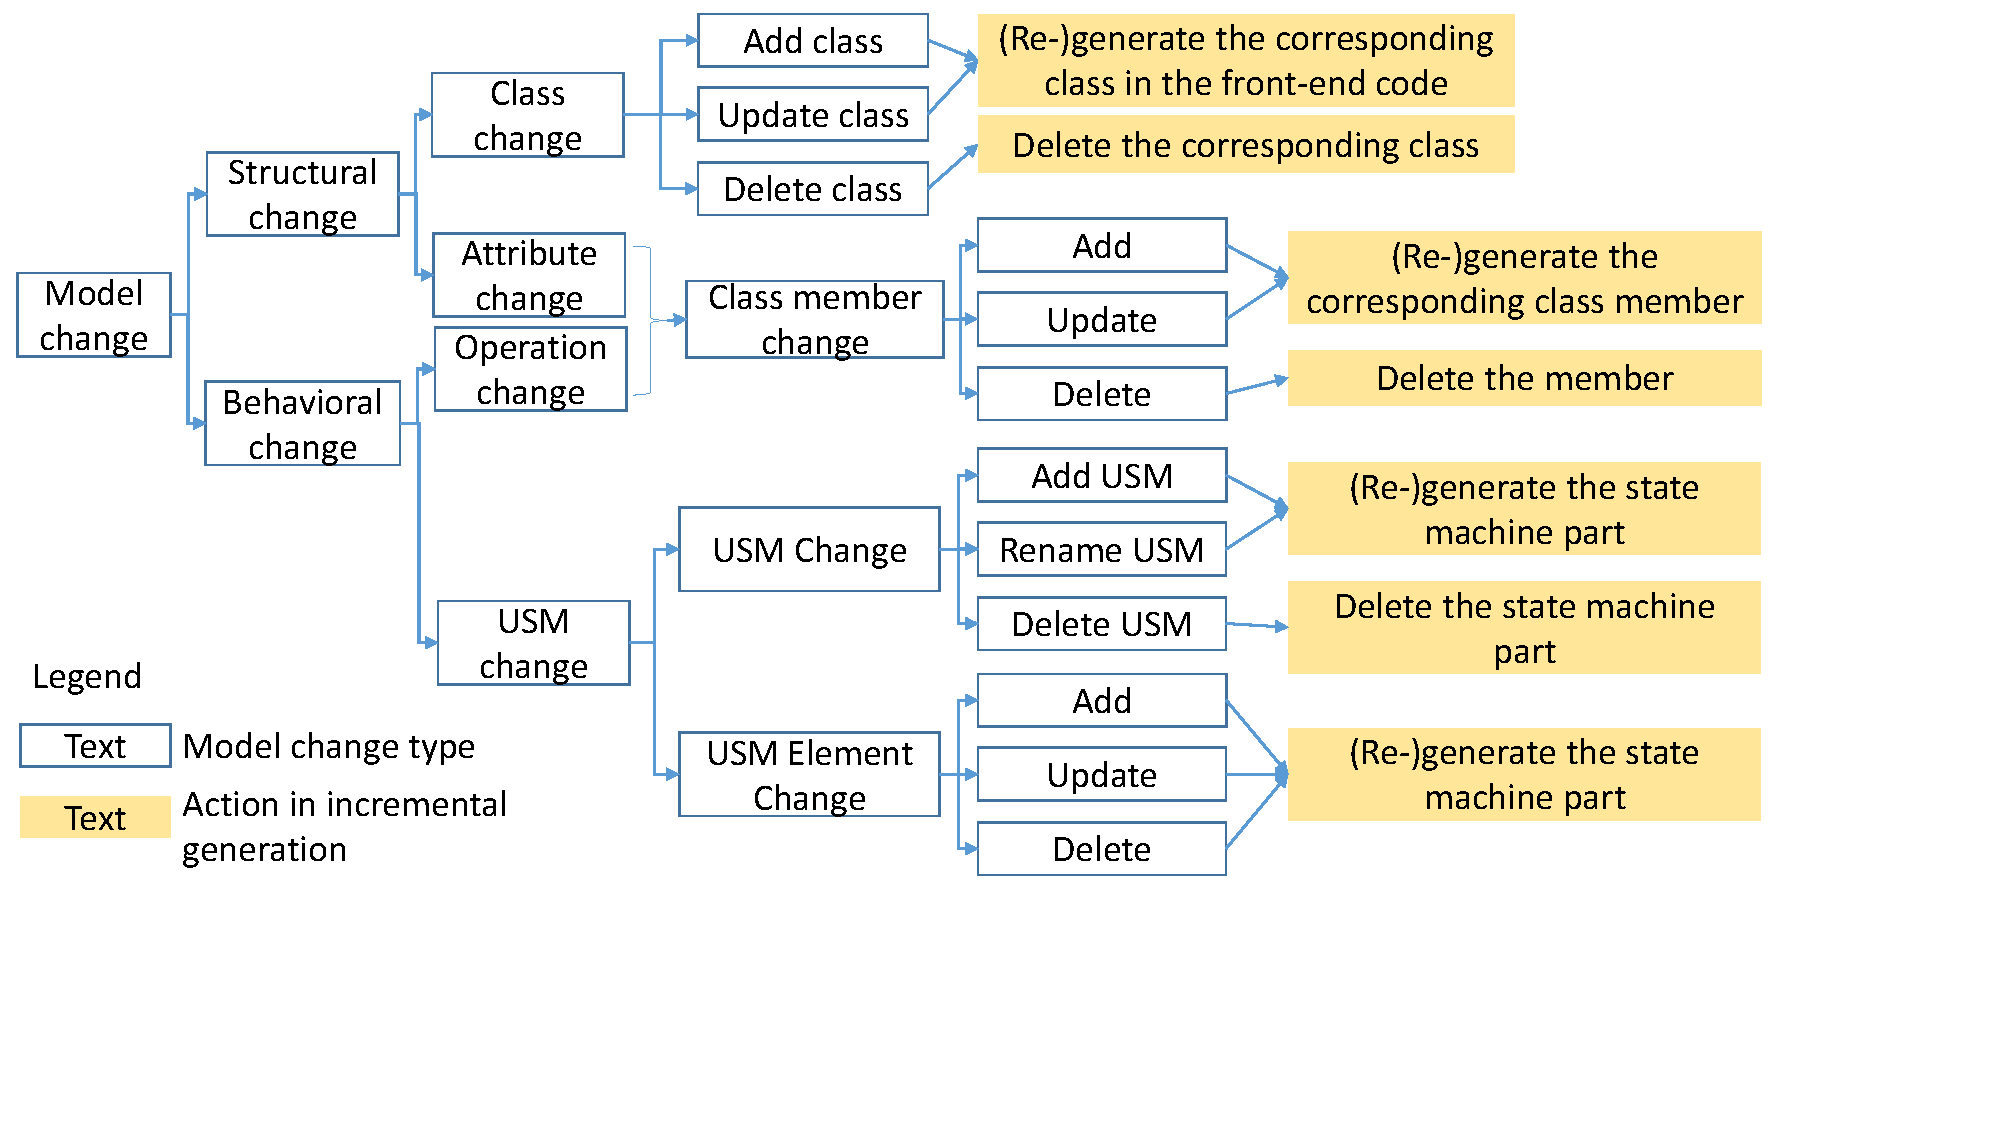
\includegraphics[clip, trim=0.2cm 4cm 4.0cm 0.2cm, width=1\columnwidth]{figures/modelchange.pdf}
	\caption{Model change management in incremental generation} 
	\label{fig:modelchange}
\end{figure}

\noindent
\paragraph{Incremental reverse engineering from front-end code to model}
%This is the inverse direction of the incremental code generator.
Similarly to the incremental code generator, there needs to be a code listener to the changes made to the code.
In Eclipse, we implemented the listener on top of C/C++ Development Tool (CDT).
The code changes are also classified as in the model change in Fig. \ref{fig:modelchange}.
The change management actions propagate the code changes to the model similarly to the other way.
Hence, we do not go to details of this implementation. 


\noindent
\paragraph{Conflict resolution strategy}


\subsection{Transformation}
The transformation takes as input the C++ front-end code to generates the C++ back-end code which is used for compilation and execution.
We implemented this transformation based on the reverse engineering as previously presented and a state machine code generation. 

Fig. \ref{fig:s2stransformation} describes the transformation is realized in two steps.
Step 1 reverse engineers the front-code to UML models with USMs and Step 2 generates the back-end code via USM code generators.
Although there are many approaches and tools supporting code generation for USMs, a complete approach is still missing \cite{Badreddin2014}, especially when considering concurrency and the support of event types.
Therefore, in order to provide full synchronization of USMs and code, we design an approach to generating code from USMs with full features to not restrict developers in modeling and coding. 

Our code generation approach combines the state pattern in \cite{niaz_mapping_2004} and IF/ELSE constructions, and extends the support of these patterns for all of pseudo states and events defined in USMs.
The detail of the generation is not presented here due to space limitation.
For example, the generated back-end code for the USM examples in Fig. \ref{fig:illustration} is shown in Fig. \ref{fig:frontend-overview}. 


\begin{figure}
	\centering
	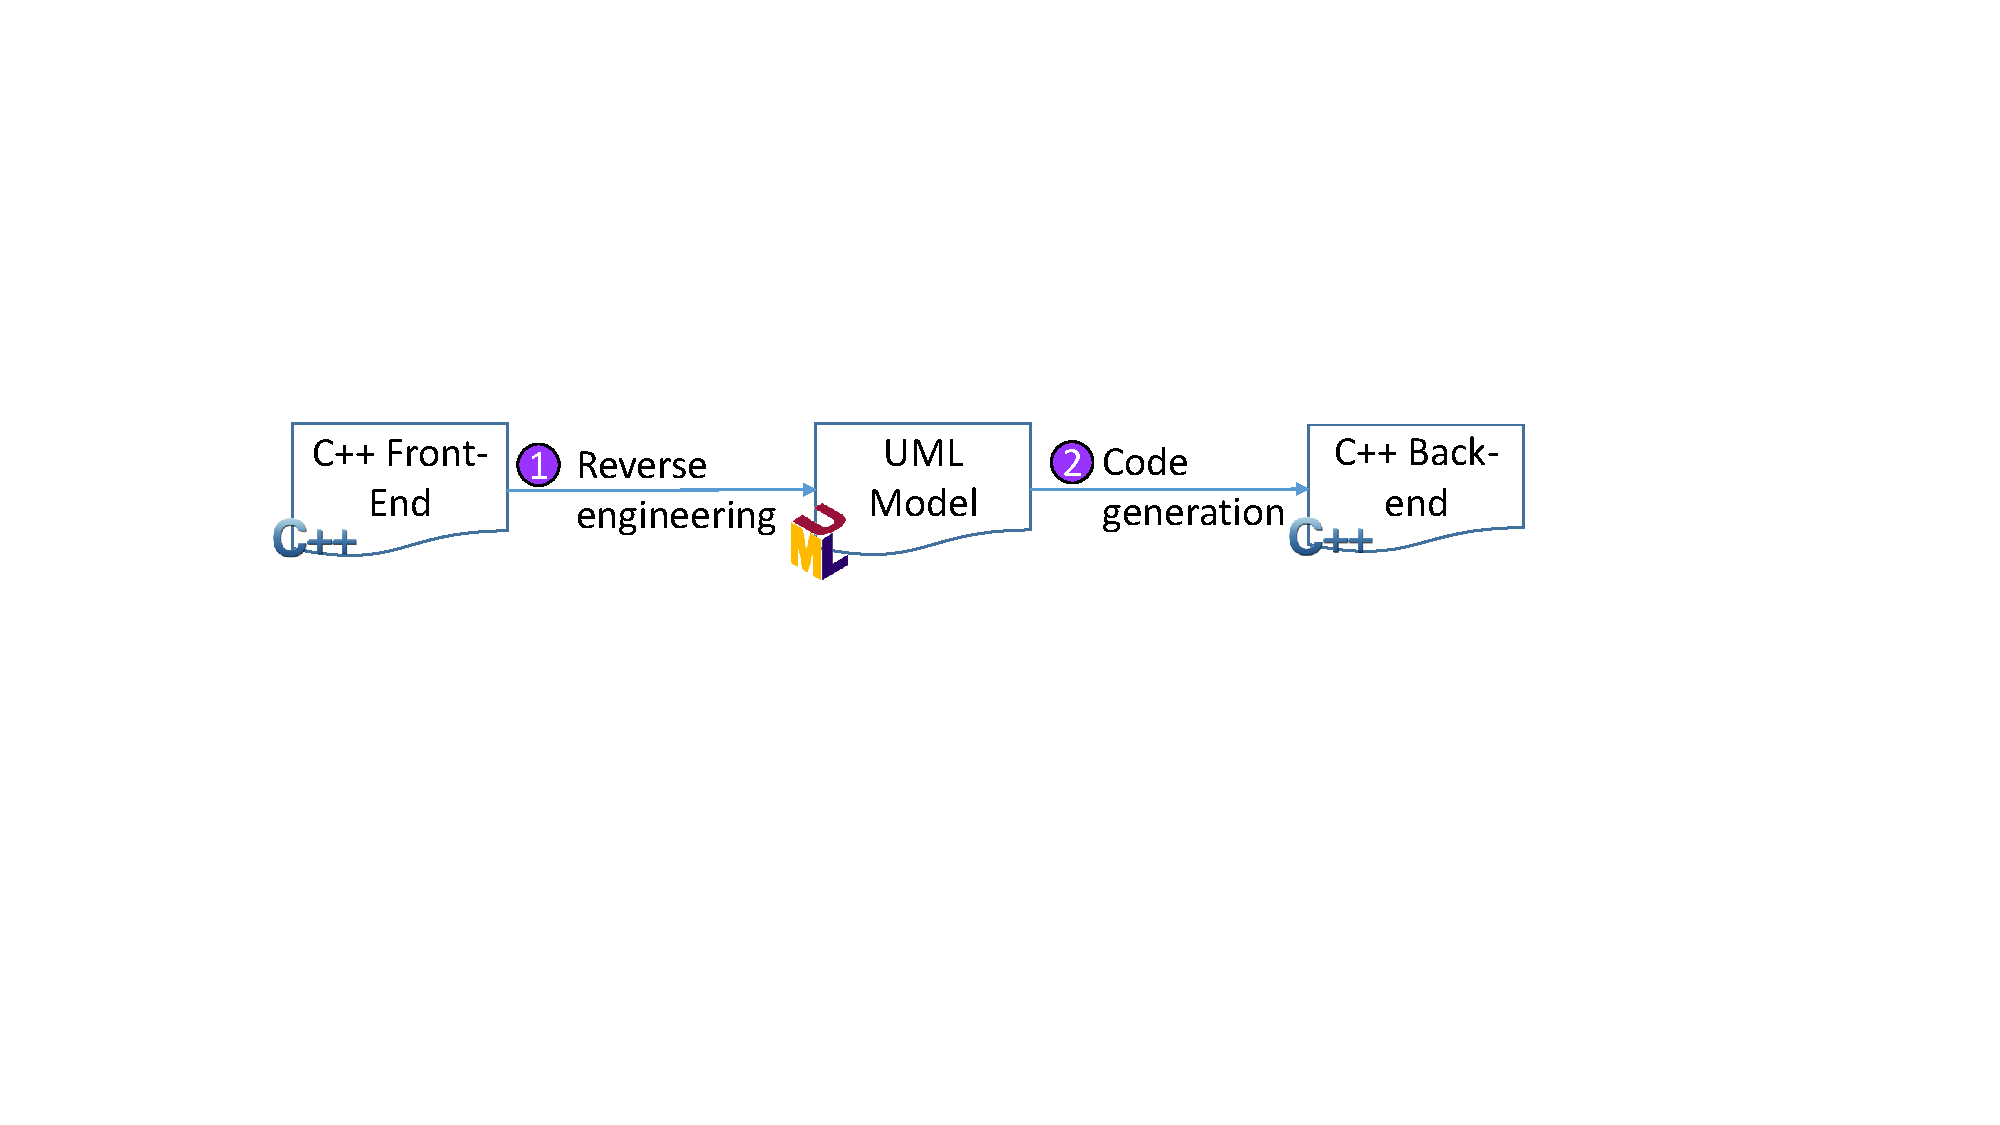
\includegraphics[clip, trim=4.5cm 9.3cm 7.7cm 7.0cm, width=1.0\columnwidth]{figures/s2stransformation.pdf}
	\caption{Source-to-source transformation via reverse engineering and code generation} 
	\label{fig:s2stransformation}
\end{figure}